\documentclass[conference]{IEEEtran}
\IEEEoverridecommandlockouts
% The preceding line is only needed to identify funding in the first footnote. If that is unneeded, please comment it out.
\usepackage{cite}
\usepackage[ngerman]{babel}
\usepackage[utf8]{inputenc}
\usepackage{amsmath,amssymb,amsfonts}
\usepackage{algorithmic}
\usepackage{graphicx}
\usepackage{textcomp}
\usepackage{xcolor}
\usepackage{listings}


\definecolor{pblue}{rgb}{0.13,0.13,1}
\definecolor{pgreen}{rgb}{0,0.5,0}
\definecolor{pred}{rgb}{0.9,0,0}
\definecolor{pgrey}{rgb}{0.46,0.45,0.48}
\lstset{language=Java,
	showspaces=false,
	showtabs=false,
	breaklines=true,
	tabsize=2,
	showstringspaces=false,
	breakatwhitespace=true,
	commentstyle=\color{pgreen},
	keywordstyle=\color{pblue},
	stringstyle=\color{pred},
	basicstyle=\ttfamily
}


\usepackage{url}
\def\BibTeX{{\rm B\kern-.05em{\sc i\kern-.025em b}\kern-.08em
		T\kern-.1667em\lower.7ex\hbox{E}\kern-.125emX}}
\begin{document}
	
	\title{Computational Geometry - Abgabe 3}
	
	\author{\IEEEauthorblockN{1\textsuperscript{st} Bartolovic Eduard}
		\IEEEauthorblockA{\textit{Hochschule München} \\
			München, Deutschland \\
			eduard.bartolovic0@hm.edu}
	}
	
	\maketitle
	
	\begin{abstract}
		
		
	\end{abstract}
	
	\section{Basis Bentley-Ottmann Algorithmus}
	PSEUDOCODE
	\begin{lstlisting}[basicstyle=\tiny]
	public double calculateArea(){
	double sum = 0;
	for(Polygon p : areas){
	boolean isInside = false;
	for(Polygon p2 : areas){
	//Check if Hole
	if(!p.equals(p2) && p.isPolygonInside(p2) ){ 
	isInside = true;
	break;
	}   
	}
	if(isInside)
	sum -= Math.abs(p.calculateArea());
	else
	sum += Math.abs(p.calculateArea());
	}
	return sum;
	}
	\end{lstlisting}
	
	Zu Beginn werden alle Start und Endpunkte aller Strecken $L_{InputStrecken}$ in eine EventQueue $Q$ eingefügt. Diese EventQueue ist eine PriorityQueue die intern die Events auf der x-Achse sortiert. Die PriorityQueue ist als ein Heap implementiert. Die Operationen besitzen deshalb auch die Komplexität:
	\begin{itemize}
		\item add: $\mathcal{O}(log(n))$
		\item poll: $\mathcal{O}(1)$
	\end{itemize}
	Die Datenstruktur für die Sweepline wird eine Map basierend auf einer Rot-Schwarz-Baum Implementierung verwendet. Dieser hat die Komplexität \cite{b1}:
	\begin{itemize}
		\item add: $\mathcal{O}(log(n))$
		\item remove: $\mathcal{O}(log(n))$
		\item contains: $\mathcal{O}(log(n))$
		\item get: $\mathcal{O}(log(n))$
	\end{itemize}
	Es gibt im regulären Bentley-Ottmann Algorithmus 3 Events(START,END,INTERSECTION).
	Zu beginn liegen nur START und END Events in $Q$.\\
	Nun wird nacheinander ein Event aus $Q$ genommen. Dieses Event wird je nach Typ behandelt.\\
	Das Event START fügt das neue Segment $S_{new}$ in die Sweepline ein.
	Es wird überprüft ob ein Segment über oder unter $S_{new}$ liegt. Sollte dies der Fall sein wird überprüft ob diese sich mit $S_{new}$ schneiden. Bei einem gefundenen Schnittpunkten wird ein neues INTERSECTION Event in $Q$ eingefügt.
	\begin{lstlisting}[basicstyle=\tiny]
	{}
	\end{lstlisting}
	Bei einem END Event endet ein Segment $S_{old}$. Es wird überprüft ob ein Segment über und unter $S_{old}$ liegt. Sollten diese existieren dann wird überprüft ob diese sich schneiden. Bei einem gefundenen Schnittpunkten wird ein neues INTERSECTION Event in $Q$ eingefügt. $S_{old}$ wird aus der Sweepline entfernt.
	\begin{lstlisting}[basicstyle=\tiny]
		{}
	\end{lstlisting}
	Bei einem INTERSECTION Event......
	
	\section{Schnittpunkt zwischen 2 Geraden }
	Da es nicht reicht nur zu Wissen das zwei geraden einen Schnittpunkt haben sondern es auch nötig ist auch dessen genaue Position zu kennen musste ein neuer ALgortithmus entwickelt werden.\\
	Hierfür wurde erstmal überprüft ob der Start- oder Endpunkt p1,q1 der Strecke s1 identisch zu einem der Punkt p2 oder q2 der Strecke s2 ist. Sollte dies der Fall sein wird direkt der gemeinsame Punkt zurückgegeben.\\
	Nun werden die beiden Strecken als Geraden behandelt. So kann man mit der Geradengleichung den Schnittpunkt der zwei Geraden berechnen.\\
	Es besteht die Möglichkeit das der Schnittpunkt S nicht existiert da beide Geraden parallel zu einander sind. In diesem Fall wären wären x und y von S unendlich. In diesem Fall wird ein Optional.empty() zurückgegeben.
	Da der Schnittpunkt S über die Geradengleichung berechnet worden ist kann es sein das dieser sich auf den Geraden von s1 und s2 befindet aber nicht auf der Strecke s1 oder s2. Deshalb muss überprüft werden ob sich der Punkt in der Bounding Box der beiden Strecken befindet. Sollte dies bei beiden der Fall sein dann ist dies der korrekte Schnittpunkt.\\
	Um numerische Fehler zu reduzieren wird bei Horizontalen und Verticalen Strecken ....
	
	\section{Probleme für den Algoritmus}
	Der Algorithmus hat Probleme wenn folgende Voraussetzungen nicht erfüllt sind:
	\begin{enumerate}
		\item x-Koordinaten der Schnitt- und Endpunkte sind paarweise verschieden
		
		\item Länge der Segmente $> 0$
		
		\item nur echte Schnittpunkte
		
		\item keine Linien parallel zur y-Achse
		
		\item keine Mehrfachschnittpunkte
		
		\item keine überlappenden Segment
	\end{enumerate}
	
	\begin{figure}[h]
		\begin{center}
			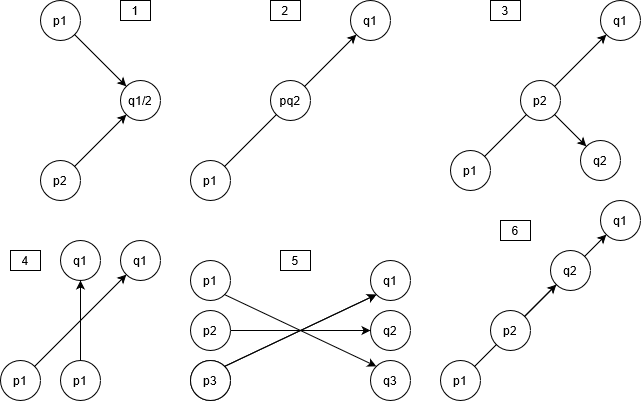
\includegraphics[width=6cm]{ProblemFaelle.png}
			\caption{Problemfälle für den Standard Bentley Ottman algorithmus}
			\label{figure_3}
		\end{center}
	\end{figure}



	\section{Behandlung der Sonderfälle}
	In meiner Implementierung wurde alle Sonderfälle behandelt.
	\subsection{Nur echte Schnittpunkte}
	Meine Implementierung unterstützt auch unechte Schnittpunkte. Hierfür wurde vor allem die Sweepline angepasst. So wird die gewöhnliche Sweepline Implementierung die nur aus einem Baum $SWEEP_{T}$ mit Strecken besteht mit einer Funktionalität ergänzt die ähnlich wie bei Buckets bei einem Hashset funktioniert. So wird bei START Events überprüft ob die Position des Startpunktes in $SWEEP_{T}$ bereits existiert. Sollte dies der Fall sein wird das Segment einfach zusätzlich in den Knoten eingefügt. Der Schlüssel der Knoten ist der aktuelle y-Wert.\\
	\begin{figure}[h!]
		\begin{center}
			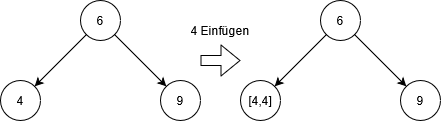
\includegraphics[width=6cm]{BaumKollision.png}
			\caption{Einfügen in die Sweepline mit Kollision}
			\label{figure_collision}
		\end{center}
	\end{figure}\\
	Leider müssen werden jedes mal wenn die Sweepline bewegt wird die Elemente in $SWEEP_{T}$ zu neu sortiert werden. Operationen auf $SWEEP_{T}$ laufen in $\mathcal{O}(n)$. 
	
	\subsection{X-Koordinaten der Schnitt- und Endpunkte sind paarweise identisch}
	Dieses Problem ist ein Teilproblem des vorherigen Problems und damit schon gelöst.
	So wird beim einfügen neuer Strecken überprüft ob bereits andere Segmente an diesem Punkt liegen. Sollte dies der Fall sein werden wird dieser Punkt entsprechend der Anzahl der Segmente als Schnittpunkte in die Output Liste eingefügt. Außerdem immer wenn ein Schnittpunkt gefunden wird welcher direkt auf der Sweepline liegt wird dieser ohne ein INTERSECTION Event zu generieren der Outputliste hinzugefügt.
	
	\subsection{Linien parallel zur Y-Achse}
	Für Linien die zur Y-Achse gehören wurden in ein neues VERTICALLINE Event erschaffen. So werden keine Startpunkt und Endpunkte in die Eventqueue eingefügt sondern nur das VERTICALLINE Event.
	Vertikale Strecken schneiden sich mit allen Strecken die aktuell die Sweepline schneiden die zwischen dem Start und Endpunkt liegen. So muss nicht die gesamte Sweepline untersucht werden sondern nur ein Teil des Baumes.
	\begin{figure}[h]
		\begin{center}
			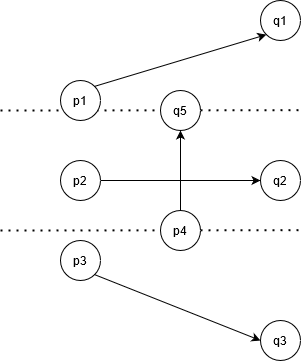
\includegraphics[width=6cm]{Vertikal.png}
			\caption{Suche nach Schnittpunkten mit Vertikalen Strecken in einem eingeschränkten Bereich}
			\label{figure_3}
		\end{center}
	\end{figure}
	Das gilt selbstverständlich auch für anderen Vertikalen Strecken an aktueller Stelle. Deshalb wird eine Vertikale Strecke auch an einem VERTICALLINE Event in die Sweepline eingefügt. Sie werden aber nicht in den Baum eingefügt sondern in eine separate Liste. Sobald die Sweepline verschoben wird werden alle vertikalen Strecken aus der Liste entfernt.
		
	\subsection{Länge der Segmente gleich $0$}
	Elemente der Länge 0 werden einfach als vertikale Linien behandelt.
	
	\subsection{Mehrfachschnittpunkte}
	Mehrfachschnittpunkte wurden behandelt. Hierfür wird die oben beschriebene Baumstruktur der Sweepline genutzt. So wird an einem INTERSECTION Event in der SweepLine gesucht ob an der Stelle weitere Segmente durchlaufen. Sollte dies der Fall sein wird werden direkt die korrekte menge an Schnittpunkten der Outputliste hinzugefügt.
	
	\subsection{Überlappende Segmente}
	Auch dieses Problem ist auch ein Teilproblem der nur echten Schnittpunkte. Dies kann aber noch mehr Probleme bereiten als das nur Überlappungen in einzelnen Punkten. Die wichtigsten Fälle in Abbildung \ref{figure_collision}.
	
	\begin{figure}[h]
		\begin{center}
			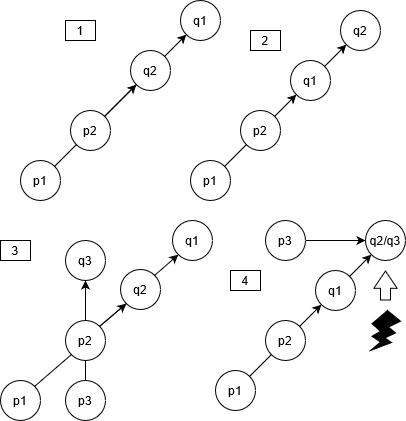
\includegraphics[width=6cm]{ProblemUberlappen.png}
			\caption{Problemfälle mit überlappenden Elementen}
			\label{figure_3}
		\end{center}
	\end{figure}
	
	\section{Komplexität}
	
	\section{Performance}
	
	\begin{enumerate}
		\item \textbf{BF S C:} BruteForce, SingleThread, nur Anzahl Schnittpunkte
		\item \textbf{BF S L:} BruteForce, SingleThread, Liste von Schnittpunkten
		\item \textbf{BF P C:} BruteForce, MultiThread, nur Anzahl Schnittpunkte
		\item \textbf{BF P L:} BruteForce, MultiThread, Liste von Schnittpunkten
		\item \textbf{BO:} Bentley-Ottmann, Liste von Schnittpunkten
	\end{enumerate}

	\begin{table}
		\small
		\begin{tabular}{|c|c|c|c|c|c|c|}
			\hline
			Datei & BF S C & BF S L & BF P C & BF P L & BO \\
			\hline
			s\_1000\_1 & 18 & 20 & 37 & 57 & 57\\
			\hline
			s\_1000\_10 & 13 & 13 & 1 & 2 & 14\\
			\hline
			s\_10000\_1 & 1263 & 1423 & 136 & 128 & 43\\
			\hline
			s\_100000\_1 & 111624 & 121718 & 8712 & 8825 & 45893\\%37363
			\hline
		\end{tabular}
	\end{table}

	Auch noch test mit 4Kerner?

	Wieso länger bei weniger Schnitt wegen voller Y-Struktur vereinzelte Same wegen sonderfälle
	
	\section{Durchschnittliche Sweeplinegröße}
	Die durchschnittliche Füllgrad der Sweepline beeinflusst die Performance.

	\begin{figure}[!tbp]
		\centering
		\begin{minipage}[b]{0.5\textwidth}
			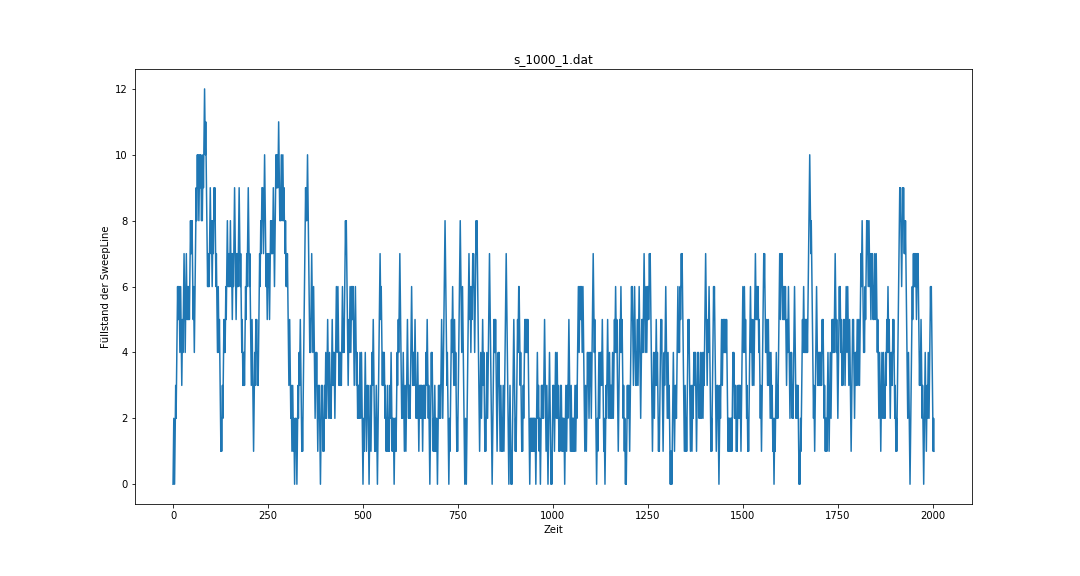
\includegraphics[width=\textwidth]{s1000+1.png}
		\end{minipage}
		\hfill
		\begin{minipage}[b]{0.5\textwidth}
			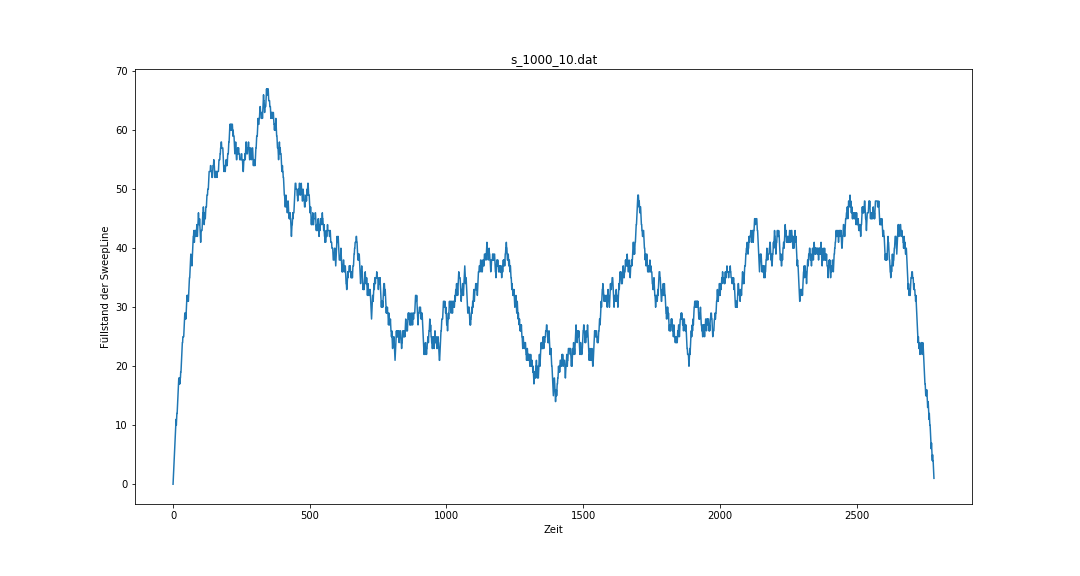
\includegraphics[width=\textwidth]{s1000+10.png}
		\end{minipage}
		\hfill
		\begin{minipage}[b]{0.5\textwidth}
			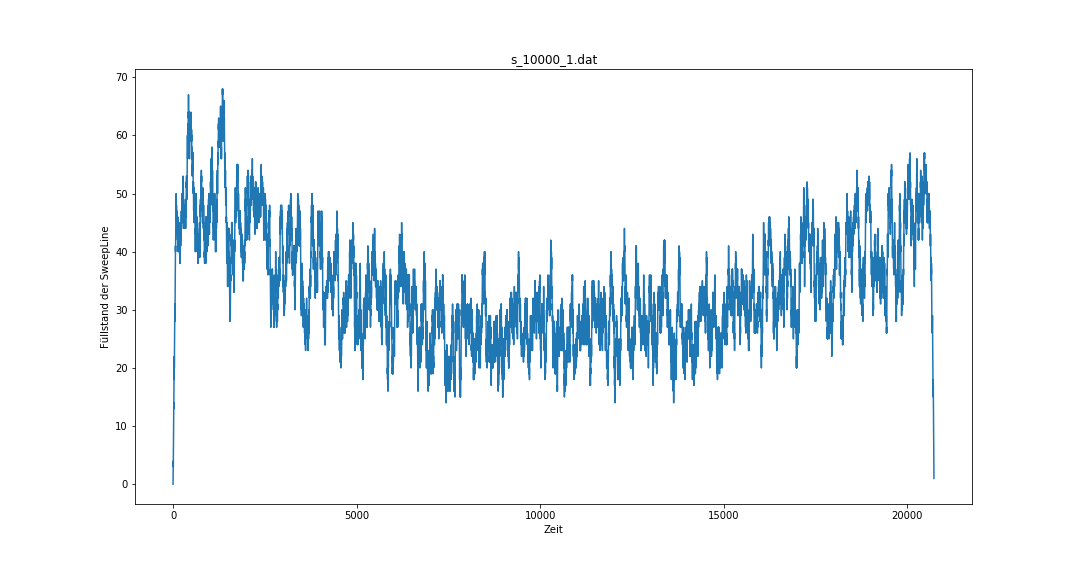
\includegraphics[width=\textwidth]{s10000+1.png}
		\end{minipage}
			\hfill
		\begin{minipage}[b]{0.5\textwidth}
			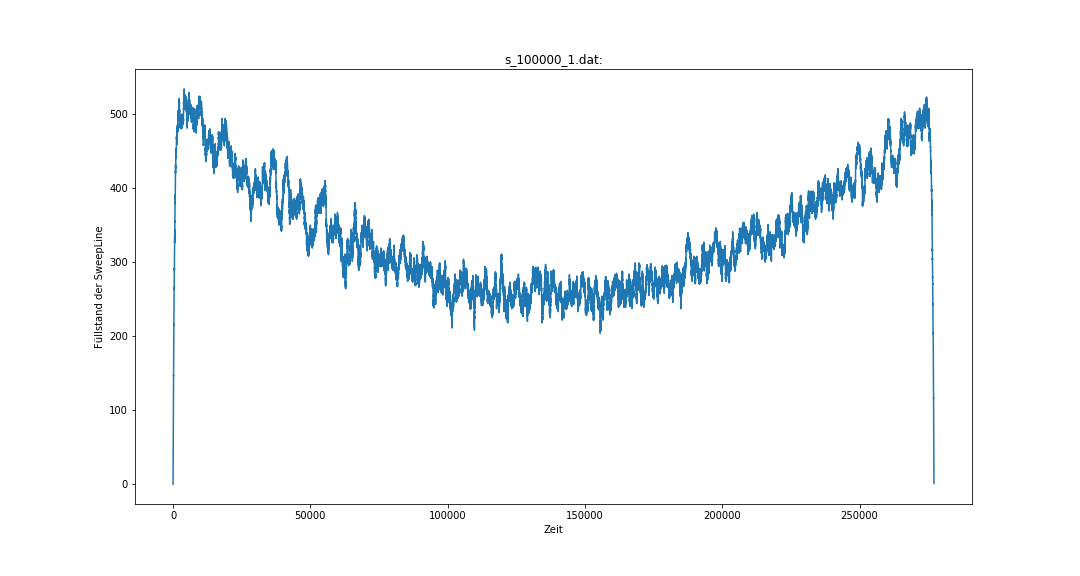
\includegraphics[width=\textwidth]{s100000+1.png}
		\end{minipage}
		\caption{Füllstand der Sweepline über die Zeit}
	\end{figure}
	
	\begin{thebibliography}{00}
		\bibitem{b1}https://docs.oracle.com/javase/7/docs/api/java/util/TreeMap.html
		\bibitem{b2}http://www.dcs.gla.ac.uk/~pat/52233/slides/Geometry1x1.pdf
	\end{thebibliography}
	
	
	
	\section{Anhang}

	Berechnung der Fläche eines Bundeslandes:
	\begin{lstlisting}[basicstyle=\tiny]
	public double calculateArea(){
		double sum = 0;
		for(Polygon p : areas){
			boolean isInside = false;
			for(Polygon p2 : areas){
				//Check if Hole
				if(!p.equals(p2) && p.isPolygonInside(p2) ){ 
					isInside = true;
					break;
				}   
			}
			if(isInside)
				sum -= Math.abs(p.calculateArea());
			else
				sum += Math.abs(p.calculateArea());
		}
		return sum;
	}
	\end{lstlisting}	

\end{document}
